\section{Simulation}
%\begin{itemize}
%	\item Simulation study is supposed to guide us to the full VARSC-model
%	\item Ideas in OneNote
%\end{itemize}

\subsection{Static Data Generating Processes}

Simulation-Procedure
\begin{itemize}
	\item \cite{abadie:2010} suppose that the counterfactuals $Y_{1,t}^{N}$ for $t > T_0$ are given by a factor model of the form $Y_{i,t}^{N} = \alpha_t + \theta_t Z_i + \lambda_t \mu_i + \epsilon_{it}$. $\alpha_t$ denotes an unknown common factor with constant loadings across panel units. $Z_i$ is a vector of observed panel-specific covariates, $\theta_t$ is a vector of unknown parameters, $\lambda_t$ is a vector of unknown common facots and $\mu_i$ are panel-specific unknown factor loadings. The unobserved transitory shocks $\epsilon_{it}$ have zero mean at the panel level. For this specific setting, \cite{abadie:2010} show that "[...] the bias of the SC-estimator can be bounded by a function that goes to zero as the number of pre-treatment periods increases." Further the number of donor units has to be fixed.
	\item \cite{ferman:2021} considers a de-meaned scenario without additional covariates. The representation of the counterfactuals therefore boils down to $Y_{i,t}^{N} = \lambda_t \mu_i + \epsilon_{it}$. Thus the counterfactual is given by the composition of the unknown panel-specific factor loadings and the unknown common factors plus the idiosyncratic shocks.
	\item We re-estimated the Tobacco Control and the Basque application and found that the inclusion of additional covariates did not improve the predictive accuracy of the SC estimator. Therefore, we follow the simulation suggestion of \cite{ferman:2021} and root our simulation in his proposed factor model without additional covariates. 
	\item Analogous to Ferman, we consider a setting with two common factors, $\lambda_{1,t}$ and $\lambda_{2,t}$. The potential outcomes for the treated unit and for the first half of the donor pool load exclusively with loading one on the first factor, the remaining donors load exclusively with loading one on the second factor. Therefore $\mu_i$ is a $(2 \times 1)$-rowvector with the first (second) entry being one and the second (first) entry being zero for the first (second) half of the donor pool.	
	\item In each simulation, we simulate a total of $T_0 + T_1$ observations, where $T_0$ represents the length of the pre- and $T_1$ the length of the post-treatment period. In order to have a simulation framework that is as close as possible to real world SC-applications, we choose $T_0 \in \left\lbrace 20,50,100\right\rbrace $ and $T_1 \in \left\lbrace 10,20,30\right\rbrace $. Further, we define the size of the donor pool as $J \in \left\lbrace 5,10,15,20,25,30\right\rbrace$.
	\item To initialize the simulation, we simulate the two common factors by drawing $T_0 + T_1$ \ac{iid}  observations from a standard normal distribution. Next, we multiply the common factors for all donors and the treatmend unit with the factor loadings $\mu_i$ and add \ac{iid} standard normal shocks. Additionally, we add panel-specific \ac{iid} standard normal intercepts such that our \ac{DGP} takes the following form: $Y_{i,t}^{N} = \gamma_i + \lambda_t \mu_i + \epsilon_{it}$. 
	\item Figure \ref{F_02} visualizes one potential \ac{DGP} with $T_0 = 20$ and $T_1 = 10$. To make the factor structure visible, we scaled the factor variance by $10^1$ and the shock variance by $10^{-1}$. Moreover, for better eyeball inspection, we added a constant treatment effect of $\delta_{1,t} = 10$ for $t > T_0$. Note that the specific nature of the treatment effect is irrelevant for our investigation. Since $Y_{1,t}^T$ is observable for $T>T_0$, we can choose an arbitrary functional form or even implement no treatment effect at all.
\end{itemize}
\phantom{space}
\begin{figure}[H]
	\centering
	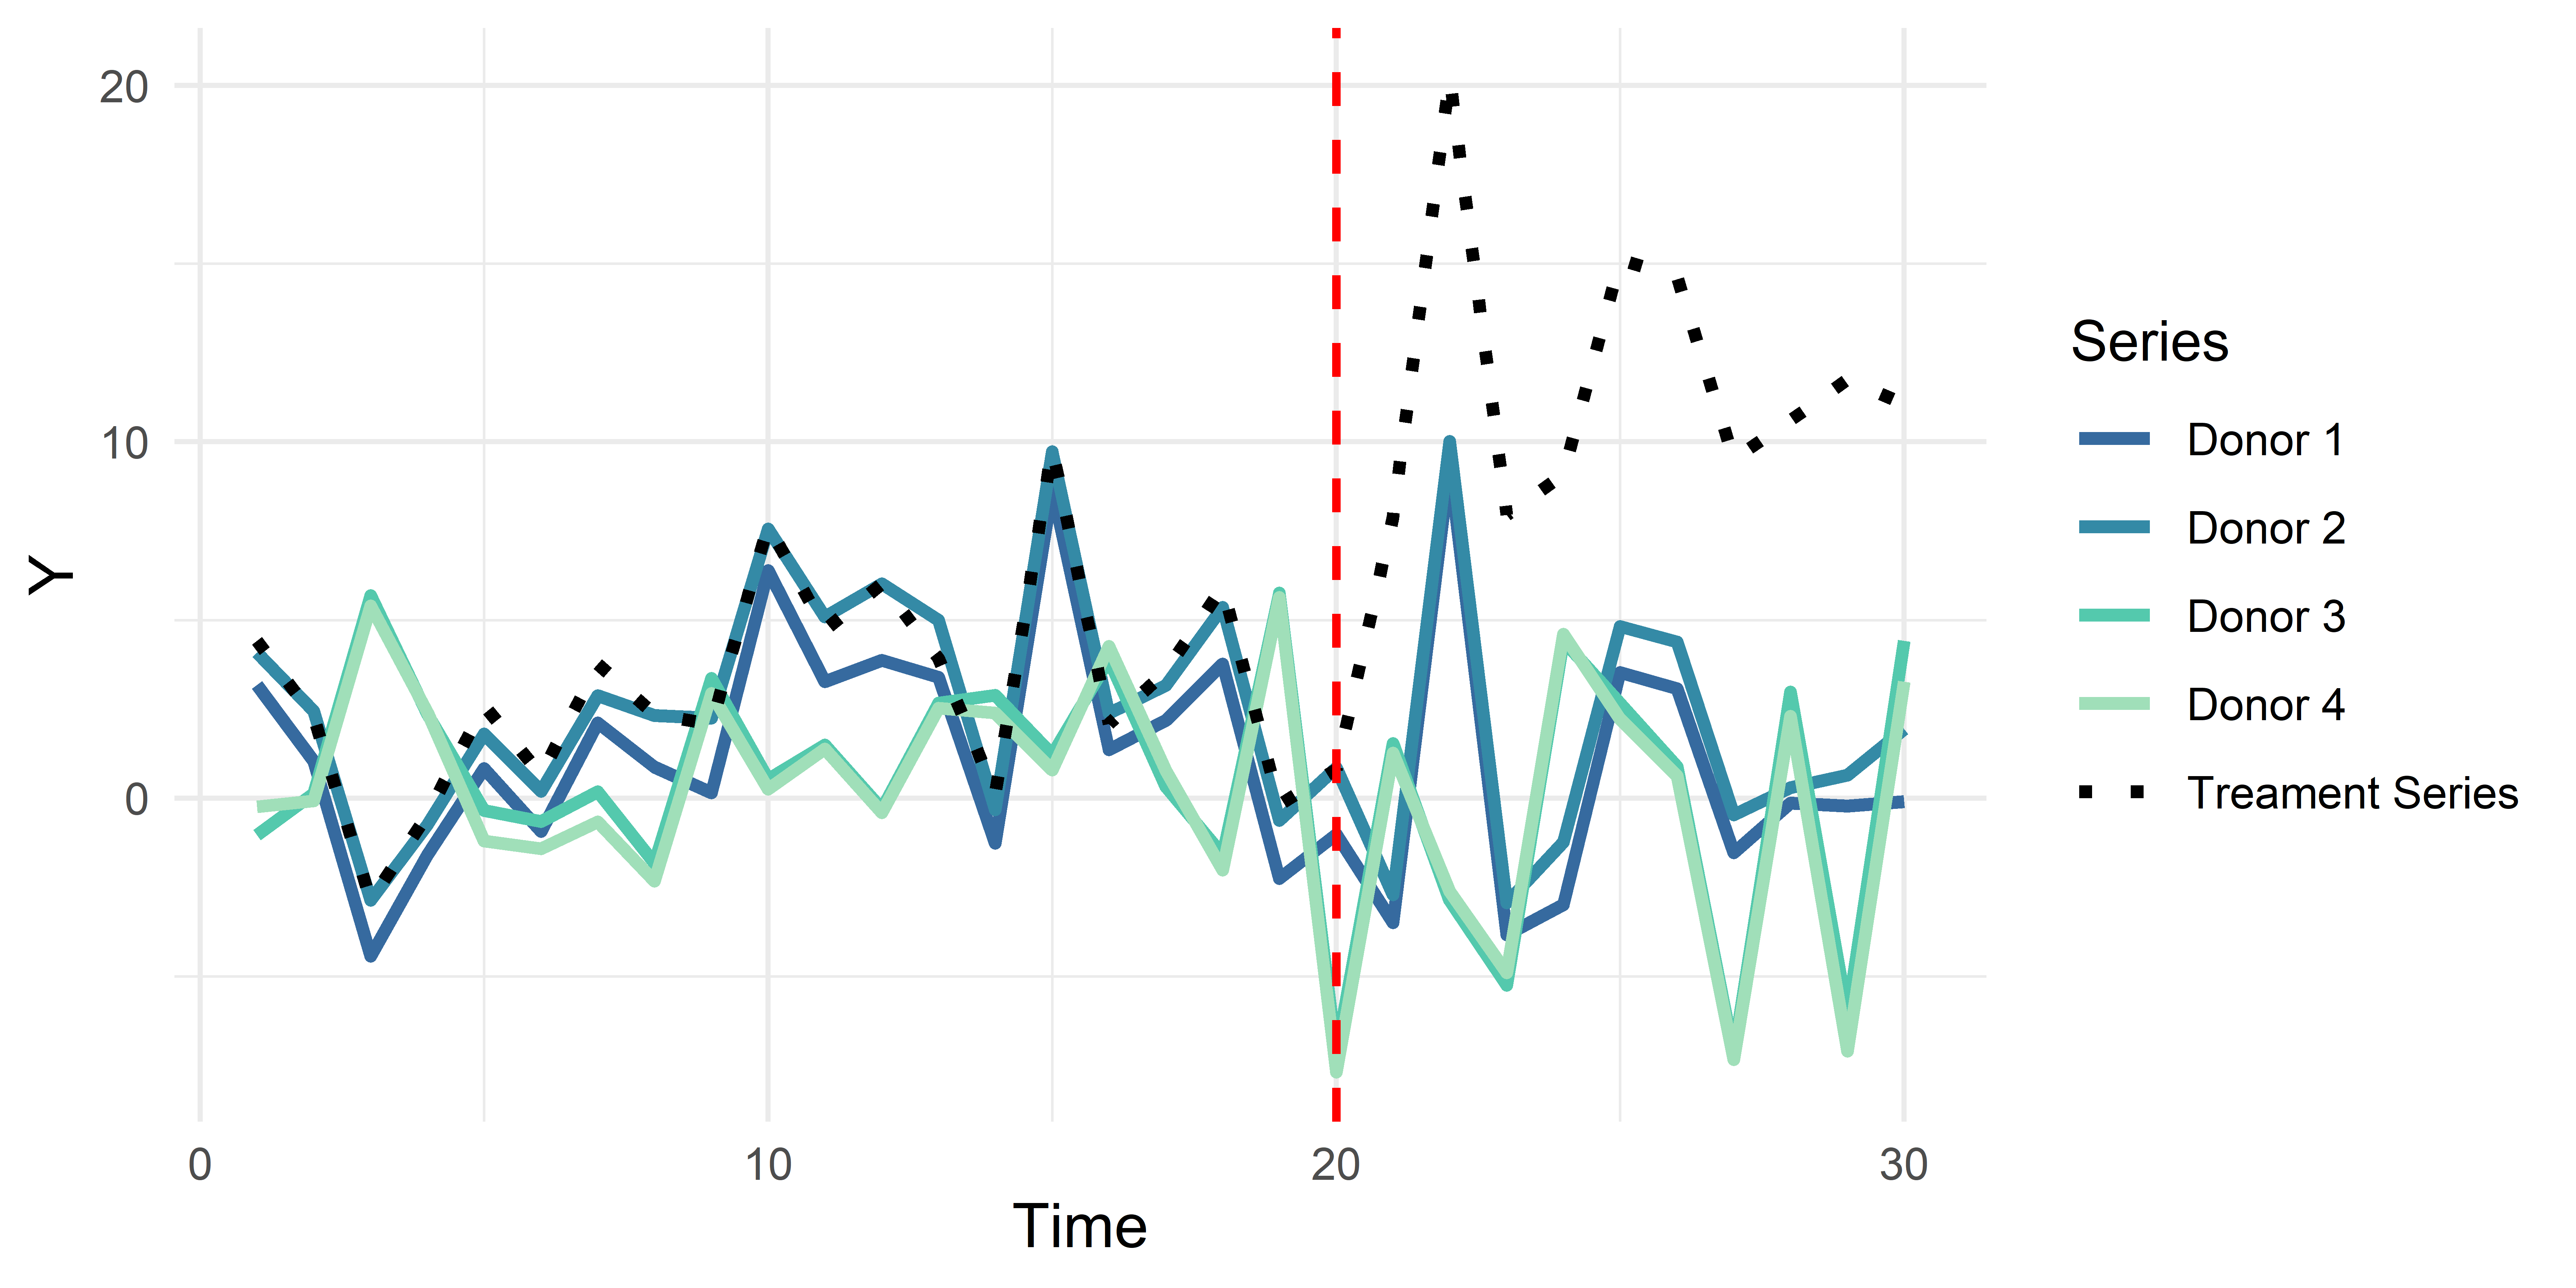
\includegraphics[scale=0.75]{F02}
	\caption{Example Factor-\ac{DGP}}
	\label{F_02}
\end{figure}
	
\begin{itemize}
	\item The described factor structure is inherent in Figure \ref{F_02}: The treatment unit and the first half of the donors (Donor\_1 and Donor\_2) as well as the second half of the donors (Donor\_3 and Donor\_4) share a common factor structure. The constant treatment effect is added after $T_0 = 20$ periods, resulting in a 10 unit vertical shift of the treatment series.
	\item We consider five different models whose goal is to recover the true factor structure of the treatment unit in the pre-treatment period and to predict the counterfactual in the post-treatment period as accurately as possible. Put differently, we train the models on $T_0$ pre-treatment observations and test their performance using $T_1$ post-treatment observations.
	\item The following models are employed: \textcolor{magenta}{\textbf{(Update when previous parts are written)}}
	\begin{enumerate}
		\item Factor-Model (FACTOR): It is assumed that the common factors and the idiosyncratic component are uncorrelated and the idiosyncratic errors are mutually uncorrelated. This suggests to estimate the common factors as linear function of the donors. A popular estimator with this property is the \ac{PC} estimator. In the training period, we obtain the predictions by regressing the treatment series on the "latent" factors. As we implemented a two-factor structure, the factors are computed by multiplying the first two eigenvalues of the covariates covariance matrix with the matrix of the covariates. The forecasts for the testing period are obtained by multiplying the factor structure of the post-treatment period with the regression coefficients of the pre-treatment regression. This model is most natural when generating data according to a factor process. Therefore, we expect it to perform best among all models.
		\item Synthetic-Control-Model (SC): In case of no additional explanatory variables, the \ac{SC}-approach reduces to a constraint regression that regresses the treatment series on the donor series given the constraint of no intercept and non-negative coefficients that sum up to one. \ac{ADH} argue that the constraints prevent the SC models from over-fitting, but they do so at the cost of a reduction in flexibility.
		\item Regularized OLS-Model (REGOLS): Our proposed model. We allow for a constant and arbitrary coefficient values. We propose a two-dimensional regularization: A ridge/l2-norm penalty that penalizes the coefficient sum and a second penalty term that shrinks the coefficient sum towards one. We identify the optimal hyperparameter-combination by applying a 50/50 train-test-split in the pre-treatment period on a two-step random grid search. In the first step, we randomly select 400 hyperparameter-combinations from a $(50 \times 50)$-grid. In the second step, we enclose the potential optimum by sequentially holding the first and the second hyperparameter fixed while increasing and decreasing the remaining hyperparameter on a coarser grid. 
		\item Elastic Net (NET): \cite{doudchenko:2016} propose to estimate the counterfactual using an elastic net regression. 
		\item OLS-Model (OLS): Finally, to verify the belief that a simple linear model overfits the training data and therefore yields poor forecasting accuracy in the testing period, we also employ an ordinary least squares model.
	\end{enumerate}
\end{itemize}

All simulations are conducted with 1,000 iterations per combination of pre- and post-treatment horizon and donor quantity.

\begin{table}[H]
	\centering
	\noindent
	\caption{Simulation Results of the Static Factor Model with \textbf{J = 5} Donors.}
	\scalebox{1}{
		\begin{tabular}{c c | C{2.4cm} | C{2.4cm} | C{2.4cm} | C{2.4cm} | C{2.4cm} }
			\toprule[1.5pt]
			\multicolumn{1}{c}{$\boldsymbol{T_0}$} & \multicolumn{1}{c}{$\boldsymbol{T_1}$}& \multicolumn{1}{c}{\textbf{FACTOR}} & \multicolumn{1}{c}{\textbf{SC}} & \multicolumn{1}{c}{\textbf{REGOLS}}& \multicolumn{1}{c}{\textbf{NET}}& \multicolumn{1}{c}{\textbf{OLS}}\\
			\cmidrule(lr){1-7}
			& & RMSE&RMSE&RMSE&RMSE&RMSE\\
			& & (BIAS)&(BIAS)&(BIAS)&(BIAS)&(BIAS)\\
			& & [VARIANCE] & [VARIANCE]& [VARIANCE]&[VARIANCE] &[VARIANCE]\\
			\cmidrule(lr){1-7}
			20&30&1.2494&1.4604&1.2942&1.2959&1.3552\\
			&&(0.0166)&(0.0001)&(0.0142)&(0.0123)&(0.0102)\\
			&&[0.6158]&[1.1078]&[0.6464]&[0.5695]&[1.1093]\\
			&20&1.2595&1.4560&1.3080&1.3067&1.3665\\
			&&(-0.0068)&(0.0320)&(-0.0009)&(-0.0003)&(0.0066)\\
			&&[0.6477]&[1.0652]&[0.6610]&[0.5948]&[1.0979]\\
			&10&1.2342&1.4322&1.2877&1.2865&1.3569\\
			&&(0.0250)&(0.0256)&(0.0256)&(0.0202)&(0.0309)\\
			&&[0.6312]&[1.0473]&[0.6361]&[0.5516]&[1.0745]\\
			\cmidrule(lr){1-7}
			% next specification
			50&30&1.1819&1.4327&1.2130&1.1987&1.2133\\
			&&(-0.0025)&(-0.0015)&(-0.0036)&(-0.0014)&(-0.0034)\\
			&&[0.6326]&[1.0579]&[0.6444]&[0.5430]&[0.7755]\\
			&20&1.1837&1.4224&1.2124&1.2046&1.2194\\
			&&(0.0092)&(0.0097)&(0.0144)&(0.0131)&(0.0150)\\
			&&[0.6469]&[1.0563]&[0.6396]&[0.5583]&[0.7840]\\
			&10&1.1663&1.3990&1.1966&1.1815&1.1968\\
			&&(0.0038)&(-0.0019)&(-0.0041)&(0.0045)&(-0.0014)\\
			&&[0.5825]&[0.9754]&[0.5731]&[0.5071]&[0.7163]\\
			\cmidrule(lr){1-7}
			% next specification
			100&30&1.1636&1.3944&1.1818&1.1746&1.1807\\
			&&(-0.0046)&(0.0176)&(-0.0060)&(-0.0052)&(-0.0057)\\
			&&[0.6505]&[1.0736]&[0.6336]&[0.5802]&[0.7192]\\
			&20&1.1684&1.3973&1.1861&1.1808&1.1862\\
			&&(-0.0009)&(0.0049)&(-0.0024)&(-0.0020)&(-0.0022)\\
			&&[0.6201]&[1.0416]&[0.5941]&[0.5488]&[0.6838]\\
			&10&1.1434&1.3686&1.1552&1.1528&1.1557\\
			&&(0.0127)&(0.0263)&(0.0114)&(0.0123)&(0.0129)\\
			&&[0.5850]&[0.9784]&[0.5811]&[0.5151]&[0.6471]\\
			\bottomrule[1.5pt]
	\end{tabular}}
	\label{table:table S.1}
\end{table}

\begin{table}[H]
	\centering
	\noindent
	\caption{Simulation Results of the Static Factor Model with \textbf{J = 10} Donors.}
	\scalebox{1}{
		\begin{tabular}{c c | C{2.4cm} | C{2.4cm} | C{2.4cm} | C{2.4cm} | C{2.4cm} }
			\toprule[1.5pt]
			\multicolumn{1}{c}{$\boldsymbol{T_0}$} & \multicolumn{1}{c}{$\boldsymbol{T_1}$}& \multicolumn{1}{c}{\textbf{FACTOR}} & \multicolumn{1}{c}{\textbf{SC}} & \multicolumn{1}{c}{\textbf{REGOLS}}& \multicolumn{1}{c}{\textbf{NET}}& \multicolumn{1}{c}{\textbf{OLS}}\\
			\cmidrule(lr){1-7}
			& & RMSE&RMSE&RMSE&RMSE&RMSE\\
			& & (BIAS)&(BIAS)&(BIAS)&(BIAS)&(BIAS)\\
			& & [VARIANCE] & [VARIANCE]& [VARIANCE]&[VARIANCE] &[VARIANCE]\\
			\cmidrule(lr){1-7}
			20&30&1.1613&1.2867&1.2304&1.2739&1.6198\\
			&&(-0.0051)&(-0.0034)&(-0.0040)&(-0.0057)&(-0.0090)\\
			&&[0.7638]&[1.0520]&[0.7474]&[0.7799]&[2.1449]\\
			&20&1.1555&1.2840&1.2250&1.2595&1.6167\\
			&&(-0.0059)&(-0.0267)&(-0.0059)&(0.0061)&(-0.0024)\\
			&&[0.7316]&[1.0055]&[0.7538]&[0.7655]&[2.1752]\\
			&10&1.1312&1.2532&1.1987&1.2395&1.5811\\
			&&(-0.0091)&(-0.0102)&(-0.0140)&(-0.0149)&(-0.0052)\\
			&&[0.6970]&[0.9745]&[0.7263]&[0.7504]&[2.0458]\\
			\cmidrule(lr){1-7}
			% next specification
			50&30&1.1043&1.2497&1.1369&1.1467&1.2086\\
			&&(0.0071)&(0.0032)&(0.0109)&(0.0111)&(0.0083)\\
			&&[0.8100]&[1.0271]&[0.7619]&[0.6834]&[1.1120]\\
			&20&1.0966&1.2308&1.1317&1.1407&1.2074\\
			&&(0.0079)&(-0.0060)&(0.0024)&(0.0063)&(0.0048)\\
			&&[0.7854]&[1.0024]&[0.7350]&[0.6546]&[1.0766]\\
			&10&1.0912&1.2167&1.1204&1.1281&1.1895\\
			&&(-0.0076)&(-0.0053)&(-0.0075)&(-0.0058)&(0.0001)\\
			&&[0.7318]&[0.9551]&[0.7016]&[0.6186]&[1.0395]\\
			\cmidrule(lr){1-7}
			% next specification
			100&30&1.0851&1.2316&1.1063&1.1112&1.1323\\
			&&(0.0065)&(0.0110)&(0.0067)&(0.0080)&(0.0081)\\
			&&[0.7875]&[1.0178]&[0.7389]&[0.6770]&[0.9248]\\
			&20&1.0733&1.2088&1.0917&1.0941&1.1202\\
			&&(-0.0137)&(0.0019)&(-0.0134)&(-0.0125)&(-0.0122)\\
			&&[0.7698]&[0.9747]&[0.7290]&[0.6631]&[0.9043]\\
			&10&1.0661&1.1986&1.0895&1.0934&1.1178\\
			&&(-0.0082)&(-0.0119)&(-0.0096)&(-0.0129)&(-0.0113)\\
			&&[0.7524]&[0.9553]&[0.7098]&[0.6451]&[0.8864]\\
			\bottomrule[1.5pt]
	\end{tabular}}
	\label{table:table S.2}
\end{table}

\begin{table}[H]
	\centering
	\noindent
	\caption{Simulation Results of the Static Factor Model with \textbf{J = 15} Donors.}
	\scalebox{1}{
		\begin{tabular}{c c | C{2.4cm} | C{2.4cm} | C{2.4cm} | C{2.4cm} | C{2.4cm} }
			\toprule[1.5pt]
			\multicolumn{1}{c}{$\boldsymbol{T_0}$} & \multicolumn{1}{c}{$\boldsymbol{T_1}$}& \multicolumn{1}{c}{\textbf{FACTOR}} & \multicolumn{1}{c}{\textbf{SC}} & \multicolumn{1}{c}{\textbf{REGOLS}}& \multicolumn{1}{c}{\textbf{NET}}& \multicolumn{1}{c}{\textbf{OLS}}\\
			\cmidrule(lr){1-7}
			& & RMSE&RMSE&RMSE&RMSE&RMSE\\
			& & (BIAS)&(BIAS)&(BIAS)&(BIAS)&(BIAS)\\
			& & [VARIANCE] & [VARIANCE]& [VARIANCE]&[VARIANCE] &[VARIANCE]\\
			\cmidrule(lr){1-7}
			20&30&1.1355&1.2504&1.2171&1.3089&2.4509\\
			&&(0.0015)&(-0.0022)&(0.0004)&(0.0012)&(0.0009)\\
			&&[0.7829]&[1.0159]&[0.7942]&[1.0400]&[6.0410]\\
			&20&1.1223&1.2368&1.2088&1.3010&2.4339\\
			&&(0.0082)&(-0.0057)&(0.0130)&(0.0024)&(0.0089)\\
			&&[0.7681]&[1.0051]&[0.8111]&[1.1466]&[6.0128]\\
			&10&1.1199&1.2299&1.2142&1.3095&2.4066\\
			&&(0.0060)&(0.0152)&(-0.0096)&(-0.0061)&(-0.0104)\\
			&&[0.7029]&[0.9262]&[0.7565]&[1.0792]&[5.7301]\\
			\cmidrule(lr){1-7}
			% next specification
			50&30&1.0834&1.2104&1.1219&1.1337&1.2756\\
			&&(0.0062)&(0.0041)&(0.0041)&(0.0041)&(0.0005)\\
			&&[0.8168]&[0.9866]&[0.7623]&[0.6970]&[1.3377]\\
			&20&1.0794&1.2016&1.1222&1.1324&1.2737\\
			&&(0.0047)&(0.0050)&(0.0043)&(0.0054)&(0.0025)\\
			&&[0.7768]&[0.9709]&[0.7428]&[0.6599]&[1.2865]\\
			&10&1.0674&1.1873&1.1010&1.1105&1.2532\\
			&&(0.0001)&(-0.0077)&(0.0021)&(0.0026)&(0.0028)\\
			&&[0.7333]&[0.8756]&[0.6879]&[0.6355]&[1.2290]\\
			\cmidrule(lr){1-7}
			% next specification
			100&30&1.0732&1.1780&1.0966&1.1032&1.1508\\
			&&(0.0036)&(0.0093)&(0.0043)&(0.0062)&(0.0059)\\
			&&[0.8262]&[0.9729]&[0.7689]&[0.6935]&[1.0253]\\
			&20&1.0645&1.1774&1.0905&1.0963&1.1459\\
			&&(-0.0153)&(-0.0091)&(-0.0185)&(-0.0192)&(-0.0203)\\
			&&[0.8304]&[0.9807]&[0.7736]&[0.7014]&[1.0300]\\
			&10&1.0627&1.1613&1.0829&1.0902&1.1378\\
			&&(0.0114)&(0.0090)&(0.0146)&(0.0149)&(0.0171)\\
			&&[0.7628]&[0.9068]&[0.7123]&[0.6393]&[0.9584]\\
			\bottomrule[1.5pt]
	\end{tabular}}
	\label{table:table S.3}
\end{table}

\begin{table}[H]
	\centering
	\noindent
	\caption{Simulation Results of the Static Factor Model with \textbf{J = 20} Donors.}
	\scalebox{1}{
		\begin{tabular}{c c | C{2.4cm} | C{2.4cm} | C{2.4cm} | C{2.4cm} | C{2.4cm} }
			\toprule[1.5pt]
			\multicolumn{1}{c}{$\boldsymbol{T_0}$} & \multicolumn{1}{c}{$\boldsymbol{T_1}$}& \multicolumn{1}{c}{\textbf{FACTOR}} & \multicolumn{1}{c}{\textbf{SC}} & \multicolumn{1}{c}{\textbf{REGOLS}}& \multicolumn{1}{c}{\textbf{NET}}& \multicolumn{1}{c}{\textbf{OLS}}\\
			\cmidrule(lr){1-7}
			& & RMSE&RMSE&RMSE&RMSE&RMSE\\
			& & (BIAS)&(BIAS)&(BIAS)&(BIAS)&(BIAS)\\
			& & [VARIANCE] & [VARIANCE]& [VARIANCE]&[VARIANCE] &[VARIANCE]\\
			\cmidrule(lr){1-7}
			20&30&1.1278&1.2332&1.2183&1.2859&NA\\
			&&(0.0020)&(-0.0040)&(-0.0039)&(-0.0079)&NA\\
			&&[0.7964]&[1.0193]&[0.8413]&[0.9901]&NA\\
			&20&1.1244&1.2312&1.2083&1.2712&NA\\
			&&(-0.0082)&(0.0043)&(-0.0054)&(0.0025)&NA\\
			&&[0.7614]&[0.9685]&[0.7839]&[0.9067]&NA\\
			&10&1.1054&1.1986&1.1987&1.2632&NA\\
			&&(0.0172)&(0.0063)&(0.0171)&(0.0169)&NA\\
			&&[0.7525]&[0.9464]&[0.8319]&[0.9309]&NA\\
			\cmidrule(lr){1-7}
			% next specification
			50&30&1.0703&1.1749&1.1087&1.1247&1.3707\\
			&&(-0.0056)&(-0.0160)&(-0.0070)&(-0.0088)&(-0.0067)\\
			&&[0.8408]&[0.9813]&[0.7851]&[0.7387]&[1.6546]\\
			&20&1.0678&1.1720&1.1117&1.1237&1.3646\\
			&&(0.0207)&(0.0202)&(0.0149)&(0.0194)&(0.0054)\\
			&&[0.8154]&[0.9649]&[0.7801]&[0.7150]&[1.5848]\\
			&10&1.0514&1.1444&1.0846&1.0976&1.3227\\
			&&(-0.0141)&(-0.0264)&(-0.0120)&(-0.0085)&(-0.0089)\\
			&&[0.7774]&[0.8997]&[0.7324]&[0.6672]&[1.4695]\\
			\cmidrule(lr){1-7}
			% next specification
			100&30&1.0447&1.1422&1.0679&1.0793&1.1626\\
			&&(-0.0039)&(0.0168)&(-0.0029)&(-0.0007)&(-0.0016)\\
			&&[0.8600]&[0.9745]&[0.7904]&[0.7231]&[1.1338]\\
			&20&1.0510&1.1476&1.0715&1.0815&1.1589\\
			&&(-0.0144)&(-0.0185)&(-0.0139)&(-0.0105)&(-0.0113)\\
			&&[0.8576]&[0.9550]&[0.7864]&[0.7234]&[1.1391]\\
			&10&1.0304&1.1144&1.0505&1.0598&1.1397\\
			&&(0.0223)&(0.0166)&(0.0271)&(0.0270)&(0.0321)\\
			&&[0.8118]&[0.9018]&[0.7425]&[0.6826]&[1.0761]\\
			\bottomrule[1.5pt]
	\end{tabular}}
	\label{table:table S.4}
\end{table}

\begin{table}[H]
	\centering
	\noindent
	\caption{Simulation Results of the Static Factor Model with \textbf{J = 25} Donors.}
	\scalebox{1}{
		\begin{tabular}{c c | C{2.4cm} | C{2.4cm} | C{2.4cm} | C{2.4cm} | C{2.4cm} }
			\toprule[1.5pt]
			\multicolumn{1}{c}{$\boldsymbol{T_0}$} & \multicolumn{1}{c}{$\boldsymbol{T_1}$}& \multicolumn{1}{c}{\textbf{FACTOR}} & \multicolumn{1}{c}{\textbf{SC}} & \multicolumn{1}{c}{\textbf{REGOLS}}& \multicolumn{1}{c}{\textbf{NET}}& \multicolumn{1}{c}{\textbf{OLS}}\\
			\cmidrule(lr){1-7}
			& & RMSE&RMSE&RMSE&RMSE&RMSE\\
			& & (BIAS)&(BIAS)&(BIAS)&(BIAS)&(BIAS)\\
			& & [VARIANCE] & [VARIANCE]& [VARIANCE]&[VARIANCE] &[VARIANCE]\\
			\cmidrule(lr){1-7}
			20&30&1.1093&NA&1.2010&1.2554&NA\\
			&&(0.0013)&NA&(0.0090)&(0.0116)&NA\\
			&&[0.7989]&NA&[0.8648]&[0.9421]&NA\\
			&20&1.1073&NA&1.1989&1.2708&NA\\
			&&(0.0131)&NA&(0.0108)&(0.0093)&NA\\
			&&[0.8177]&NA&[0.8516]&[0.9724]&NA\\
			&10&1.0971&NA&1.1928&1.2447&NA\\
			&&(-0.0046)&NA&(-0.0001)&(0.0013)&NA\\
			&&[0.7589]&NA&[0.8153]&[0.8945]&NA\\
			\cmidrule(lr){1-7}
			% next specification
			50&30&1.0597&1.1582&1.0996&1.1172&1.4863\\
			&&(-0.0018)&(0.0135)&(-0.0048)&(-0.0079)&(-0.0151)\\
			&&[0.8466]&[0.9590]&[0.7879]&[0.7353]&[1.9825]\\
			&20&1.0538&1.1525&1.0993&1.1139&1.4811\\
			&&(-0.0150)&(0.0043)&(-0.0082)&(-0.0101)&(0.0033)\\
			&&[0.8350]&[0.9332]&[0.7821]&[0.7263]&[1.9856]\\
			&10&1.0432&1.1428&1.0831&1.0997&1.4400\\
			&&(0.0062)&(-0.0038)&(0.0062)&(0.0064)&(-0.0066)\\
			&&[0.8077]&[0.9111]&[0.7625]&[0.7214]&[1.8603]\\
			\cmidrule(lr){1-7}
			% next specification
			100&30&1.0378&1.1232&1.0641&1.0741&1.1959\\
			&&(0.0000)&(0.0058)&(-0.0003)&(0.0006)&(0.0044)\\
			&&[0.8501]&[0.9454]&[0.7912]&[0.7149]&[1.2244]\\
			&20&1.0483&1.1401&1.0747&1.0842&1.2002\\
			&&(0.0110)&(0.0130)&(0.0114)&(0.0127)&(0.0147)\\
			&&[0.8655]&[0.9457]&[0.7968]&[0.7234]&[1.2330]\\
			&10&1.0296&1.1154&1.0551&1.0648&1.1811\\
			&&(-0.0018)&(-0.0017)&(-0.0012)&(0.0001)&(-0.0040)\\
			&&[0.8083]&[0.8879]&[0.7444]&[0.6782]&[1.1463]\\
			\bottomrule[1.5pt]
	\end{tabular}}
	\label{table:table S.5}
\end{table}

\begin{table}[H]
	\centering
	\noindent
	\caption{Simulation Results of the Static Factor Model with \textbf{J = 30} Donors.}
	\scalebox{1}{
		\begin{tabular}{c c | C{2.4cm} | C{2.4cm} | C{2.4cm} | C{2.4cm} | C{2.4cm} }
			\toprule[1.5pt]
			\multicolumn{1}{c}{$\boldsymbol{T_0}$} & \multicolumn{1}{c}{$\boldsymbol{T_1}$}& \multicolumn{1}{c}{\textbf{FACTOR}} & \multicolumn{1}{c}{\textbf{SC}} & \multicolumn{1}{c}{\textbf{REGOLS}}& \multicolumn{1}{c}{\textbf{NET}}& \multicolumn{1}{c}{\textbf{OLS}}\\
			\cmidrule(lr){1-7}
			& & RMSE&RMSE&RMSE&RMSE&RMSE\\
			& & (BIAS)&(BIAS)&(BIAS)&(BIAS)&(BIAS)\\
			& & [VARIANCE] & [VARIANCE]& [VARIANCE]&[VARIANCE] &[VARIANCE]\\
			\cmidrule(lr){1-7}
			20&30&1.1013&NA&1.1899&1.2523&NA\\
			&&(0.0128)&NA&(0.0149)&(0.0115)&NA\\
			&&[0.8224]&NA&[0.8865]&[0.9715]&NA\\
			&20&1.1043&NA&1.1825&1.2442&NA\\
			&&(0.0014)&NA&(0.0031)&(0.0052)&NA\\
			&&[0.8072]&NA&[0.8431]&[0.9420]&NA\\
			&10&1.0890&NA&1.1647&1.2337&NA\\
			&&(-0.0075)&NA&(-0.0054)&(-0.0055)&NA\\
			&&[0.7761]&NA&[0.8107]&[0.8943]&NA\\
			\cmidrule(lr){1-7}
			% next specification
			50&30&1.0622&1.1477&1.1039&1.1297&1.6851\\
			&&(-0.0022)&(0.0062)&(0.0009)&(-0.0012)&(0.0059)\\
			&&[0.8658]&[0.9630]&[0.8137]&[0.7852]&[2.6638]\\
			&20&1.0508&1.1372&1.0936&1.1190&1.6716\\
			&&(-0.0016)&(-0.0084)&(-0.0009)&(-0.0004)&(-0.0006)\\
			&&[0.8700]&[0.9523]&[0.8184]&[0.7841]&[2.5964]\\
			&10&1.0445&1.1342&1.0880&1.1061&1.6681\\
			&&(0.0006)&(-0.0043)&(0.0052)&(0.0091)&(0.0174)\\
			&&[0.8279]&[0.9218]&[0.7784]&[0.7648]&[2.5590]\\
			\cmidrule(lr){1-7}
			% next specification
			100&30&1.0420&1.1178&1.0662&1.0793&1.2394\\
			&&(0.0097)&(0.0172)&(0.0107)&(0.0094)&(0.0070)\\
			&&[0.8864]&[0.9693]&[0.8258]&[0.7565]&[1.3694]\\
			&20&1.0435&1.1237&1.0669&1.0788&1.2351\\
			&&(0.0072)&(0.0038)&(0.0054)&(0.0057)&(0.0064)\\
			&&[0.8778]&[0.9520]&[0.8077]&[0.7417]&[1.3400]\\
			&10&1.0159&1.0890&1.0410&1.0465&1.2026\\
			&&(0.0027)&(0.0173)&(0.0041)&(0.0020)&(0.0038)\\
			&&[0.8381]&[0.8876]&[0.7678]&[0.7076]&[1.2823]\\
			\bottomrule[1.5pt]
	\end{tabular}}
	\label{table:table S.6}
\end{table}

\subsection{Weakly Dynamic Data Generating Processes}
\subsection{Dynamic Data Generating Processes}